\section{Experiment}
\label{experiment}


\subsection{Network Setup and Launch Attack}

This section presents our experimental testing environment and the steps taken to establish it. All experiments were performed on VMware workstation 12 on live development server with the configuration 
Intel(R) Core (TM) i7-6500U CPU @ 2.50GHz, 30GB HDD, 2GB RAM for all virtual machines, and the operating system platform is Ubuntu 14.04.5 LTS Desktop 64-bit. We have installed and configured three Virtual 
Machines - ''Victim,'' ''Attacker,'' and ''Vulnerable.'' All virtual machines are run on the same individual server, but they are separate in logical. The ''victim's'' VM configured with Snort, the 
attacker's machine contains Metasploit tool-kit and we used existing
vulnerable Ubuntu operating system for testing purposes and make it as our third machine - vulnerable \cite{misc:metasploitable}. 

We have deployed and tested ten different Metasploit attacks: Port
Scanning, DoS/ TCP SYN flood, OpenSSH Exploit via NFS Service, Remote Code Execution (Ruby DRb RMI), Remote Procedure Calls (RPC) (JAVA RMI Registry), WordPress XMLRPC DoS, VSFTPD v2.3.4 Backdoor Command
Execution, Apache Exploit via PHP CGI, Anonymous login (Samba client) backdoor exploit, and Unrealircd 3.2.8.1 backdoor command execution. These attacks can be categorized into three core categories: Port
Scanning (Probe) - gathering network information to bypass security, Denial of Service (Dos) - where some resource is swamped; causing DoS to legitimate users, Remote to local (R2L) - attacks that exploit
remote system vulnerabilities to get access to a system. After successfully tested we made all of them as automated handled by Metasploit script, which we used for development of attacker's system
\cite{misc:metasploitScripts}.

%The traffic flow between each machines are shown in Figure \ref{fig:connectionModel}.

%\begin{figure}[h!]
%	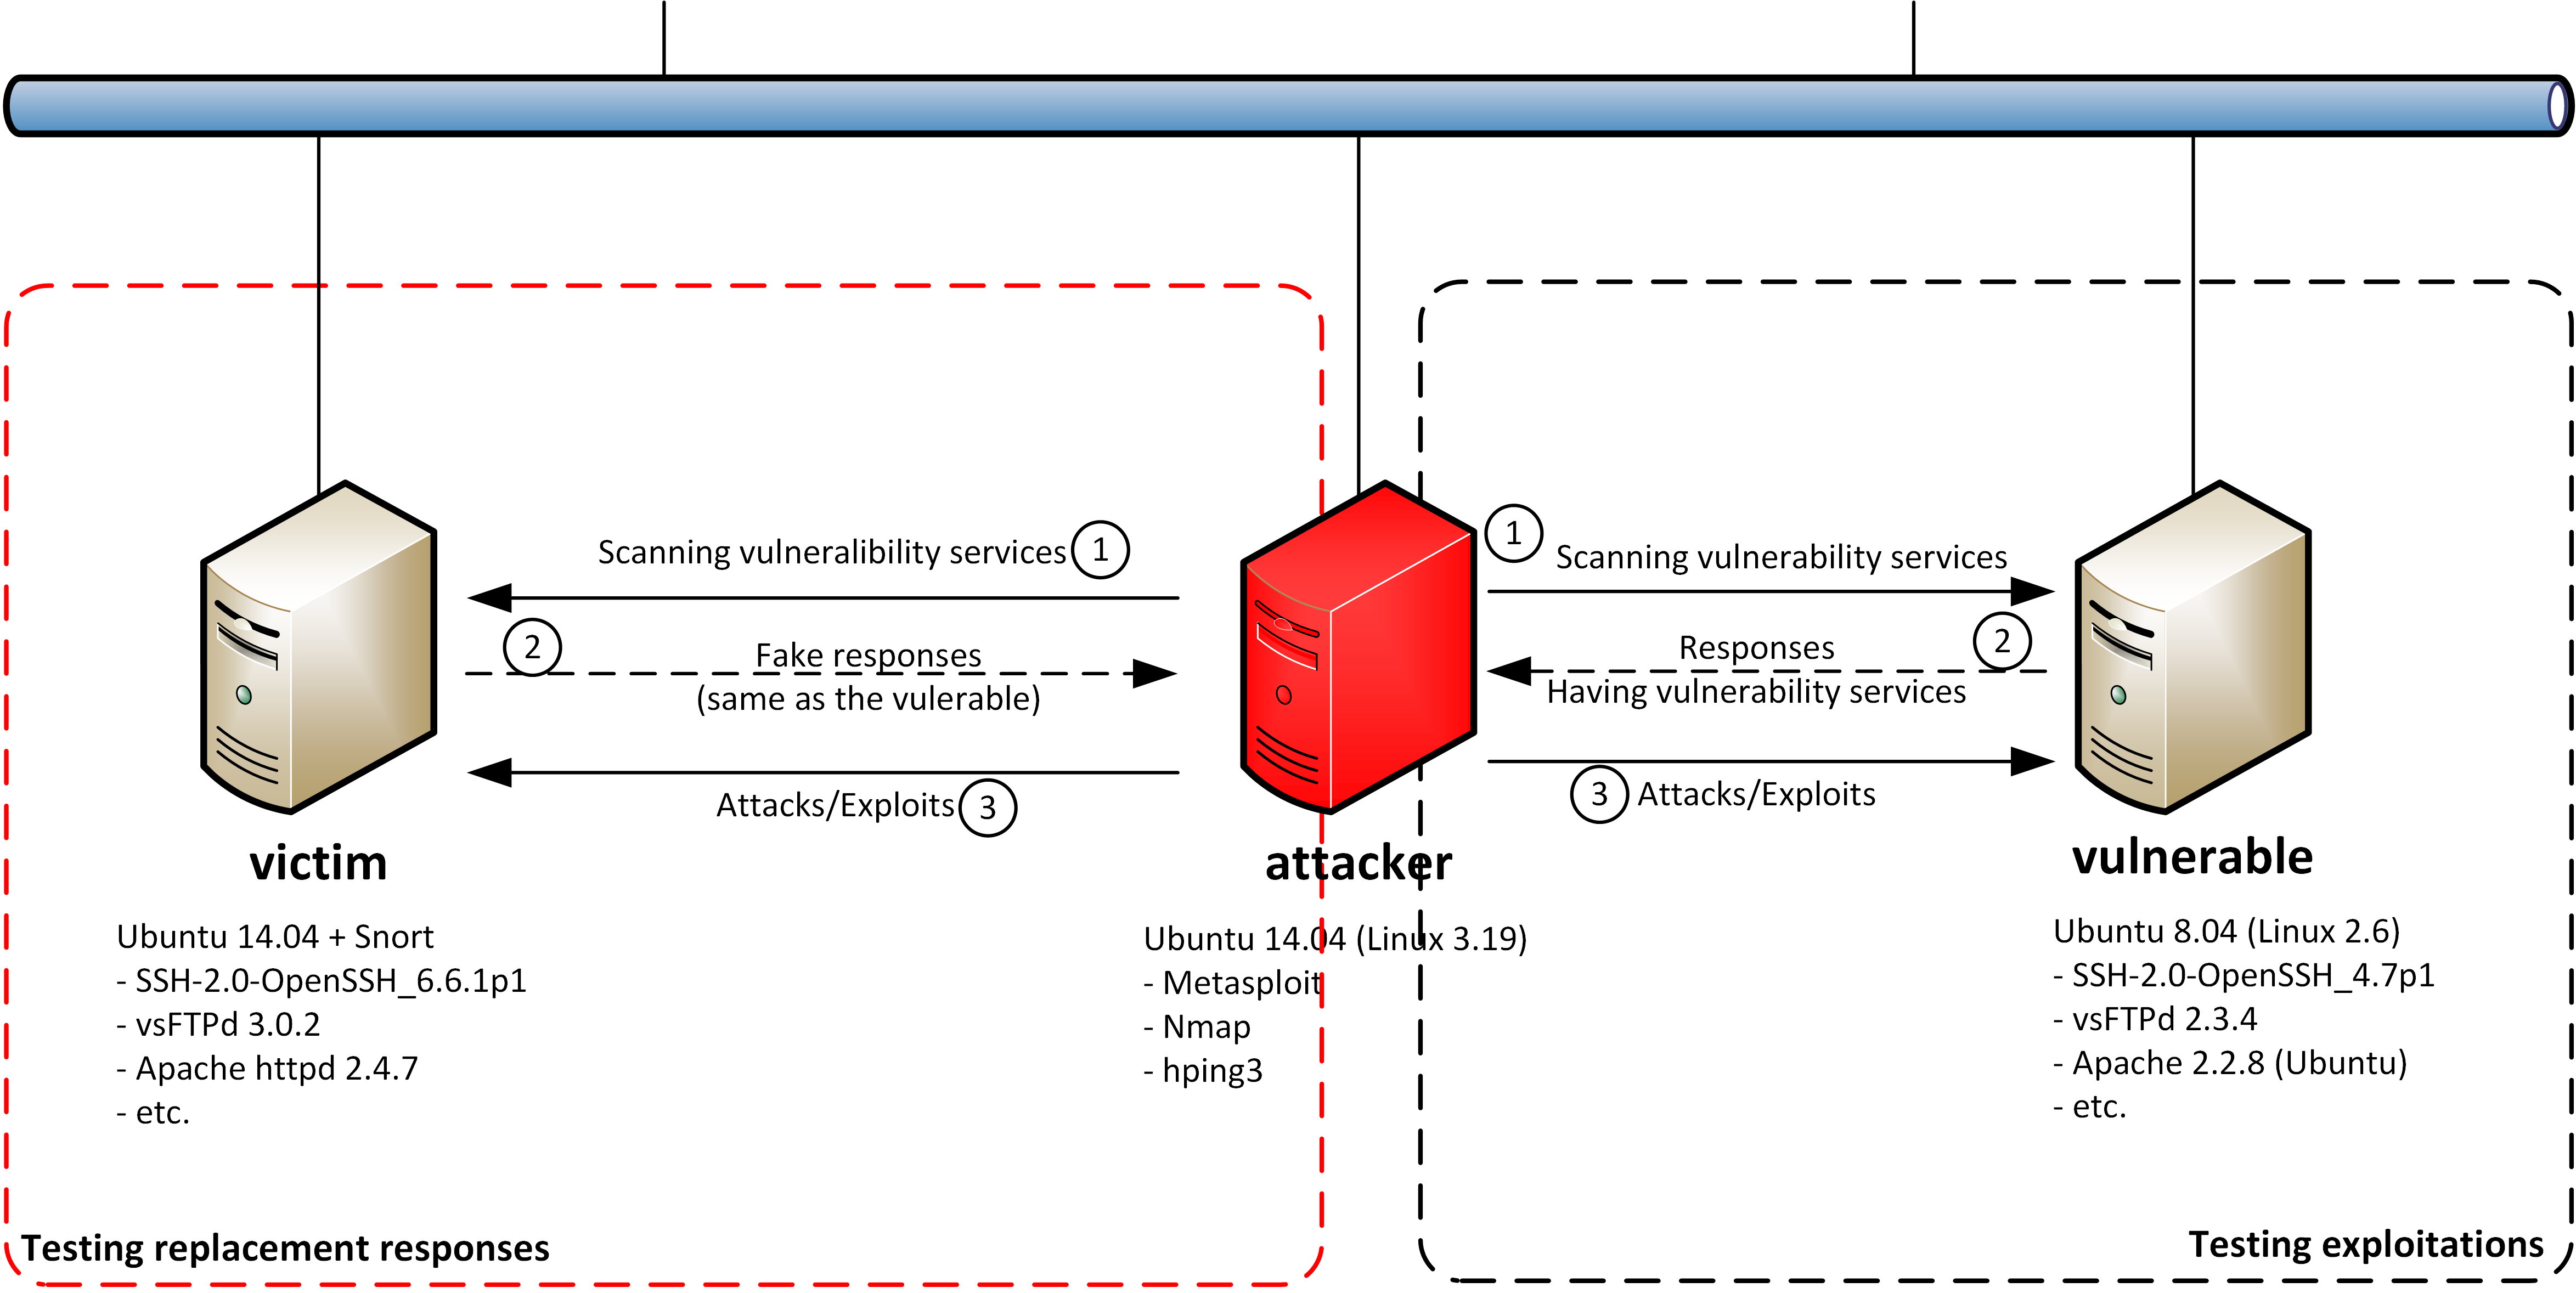
\includegraphics[width=\linewidth]{networkSecurityResearch_new_no_back.png}
%	\caption{Logical connection model}
%	\label{fig:connectionModel}
%\end{figure}

\subsection{Dataset preparation}

%We started research to work on dataset preparation by taking existing dataset and run their suggested machine learning techniques using weka tool. And when we were %working on KDD- cup'99 dataset we found
%it was really outdated as it was to older and those number of features which they have focused on, it was not applicable with %our research because we focused on network threat as we were looking at
%network behavior and traffic for anomaly detection for intrusion detection %system\cite{anomaly-basedNID}.

In this part of research to collect and extract dataset we started data modeling with existing different labeled datasets to understand the model of machine learning. Then we worked on existing datasets to
extract usable features from them and we came up with the java parser script which can parse and extract entire data information from Pcap file and saved into Csv file. We put time-window size variable to
extract and identify unique combinations of packet transmission. Parser can parse and split the entire Pcap information with respect to the time-window size, as this feature is flexible and it depend on the nodes in our network. While researching on previous suggested
approaches we tried to extract the dataset in different time-windows sizes: 10 seconds, 1 seconds, 7 seconds, and 5 seconds. We observe that 4 second time frame is more preferable in our
network architecture as it generates more accurate results with weka. We collected and built our own datasets to test our model and
accuracy of algorithms for anomaly detection of network attacks \cite{DMnIDS}. We launch each attack repeatedly and capture them in PCAP format. We extract them into CSV format using a 4 second time window format using ourown CSV-parser.

\begin{figure}[h!]
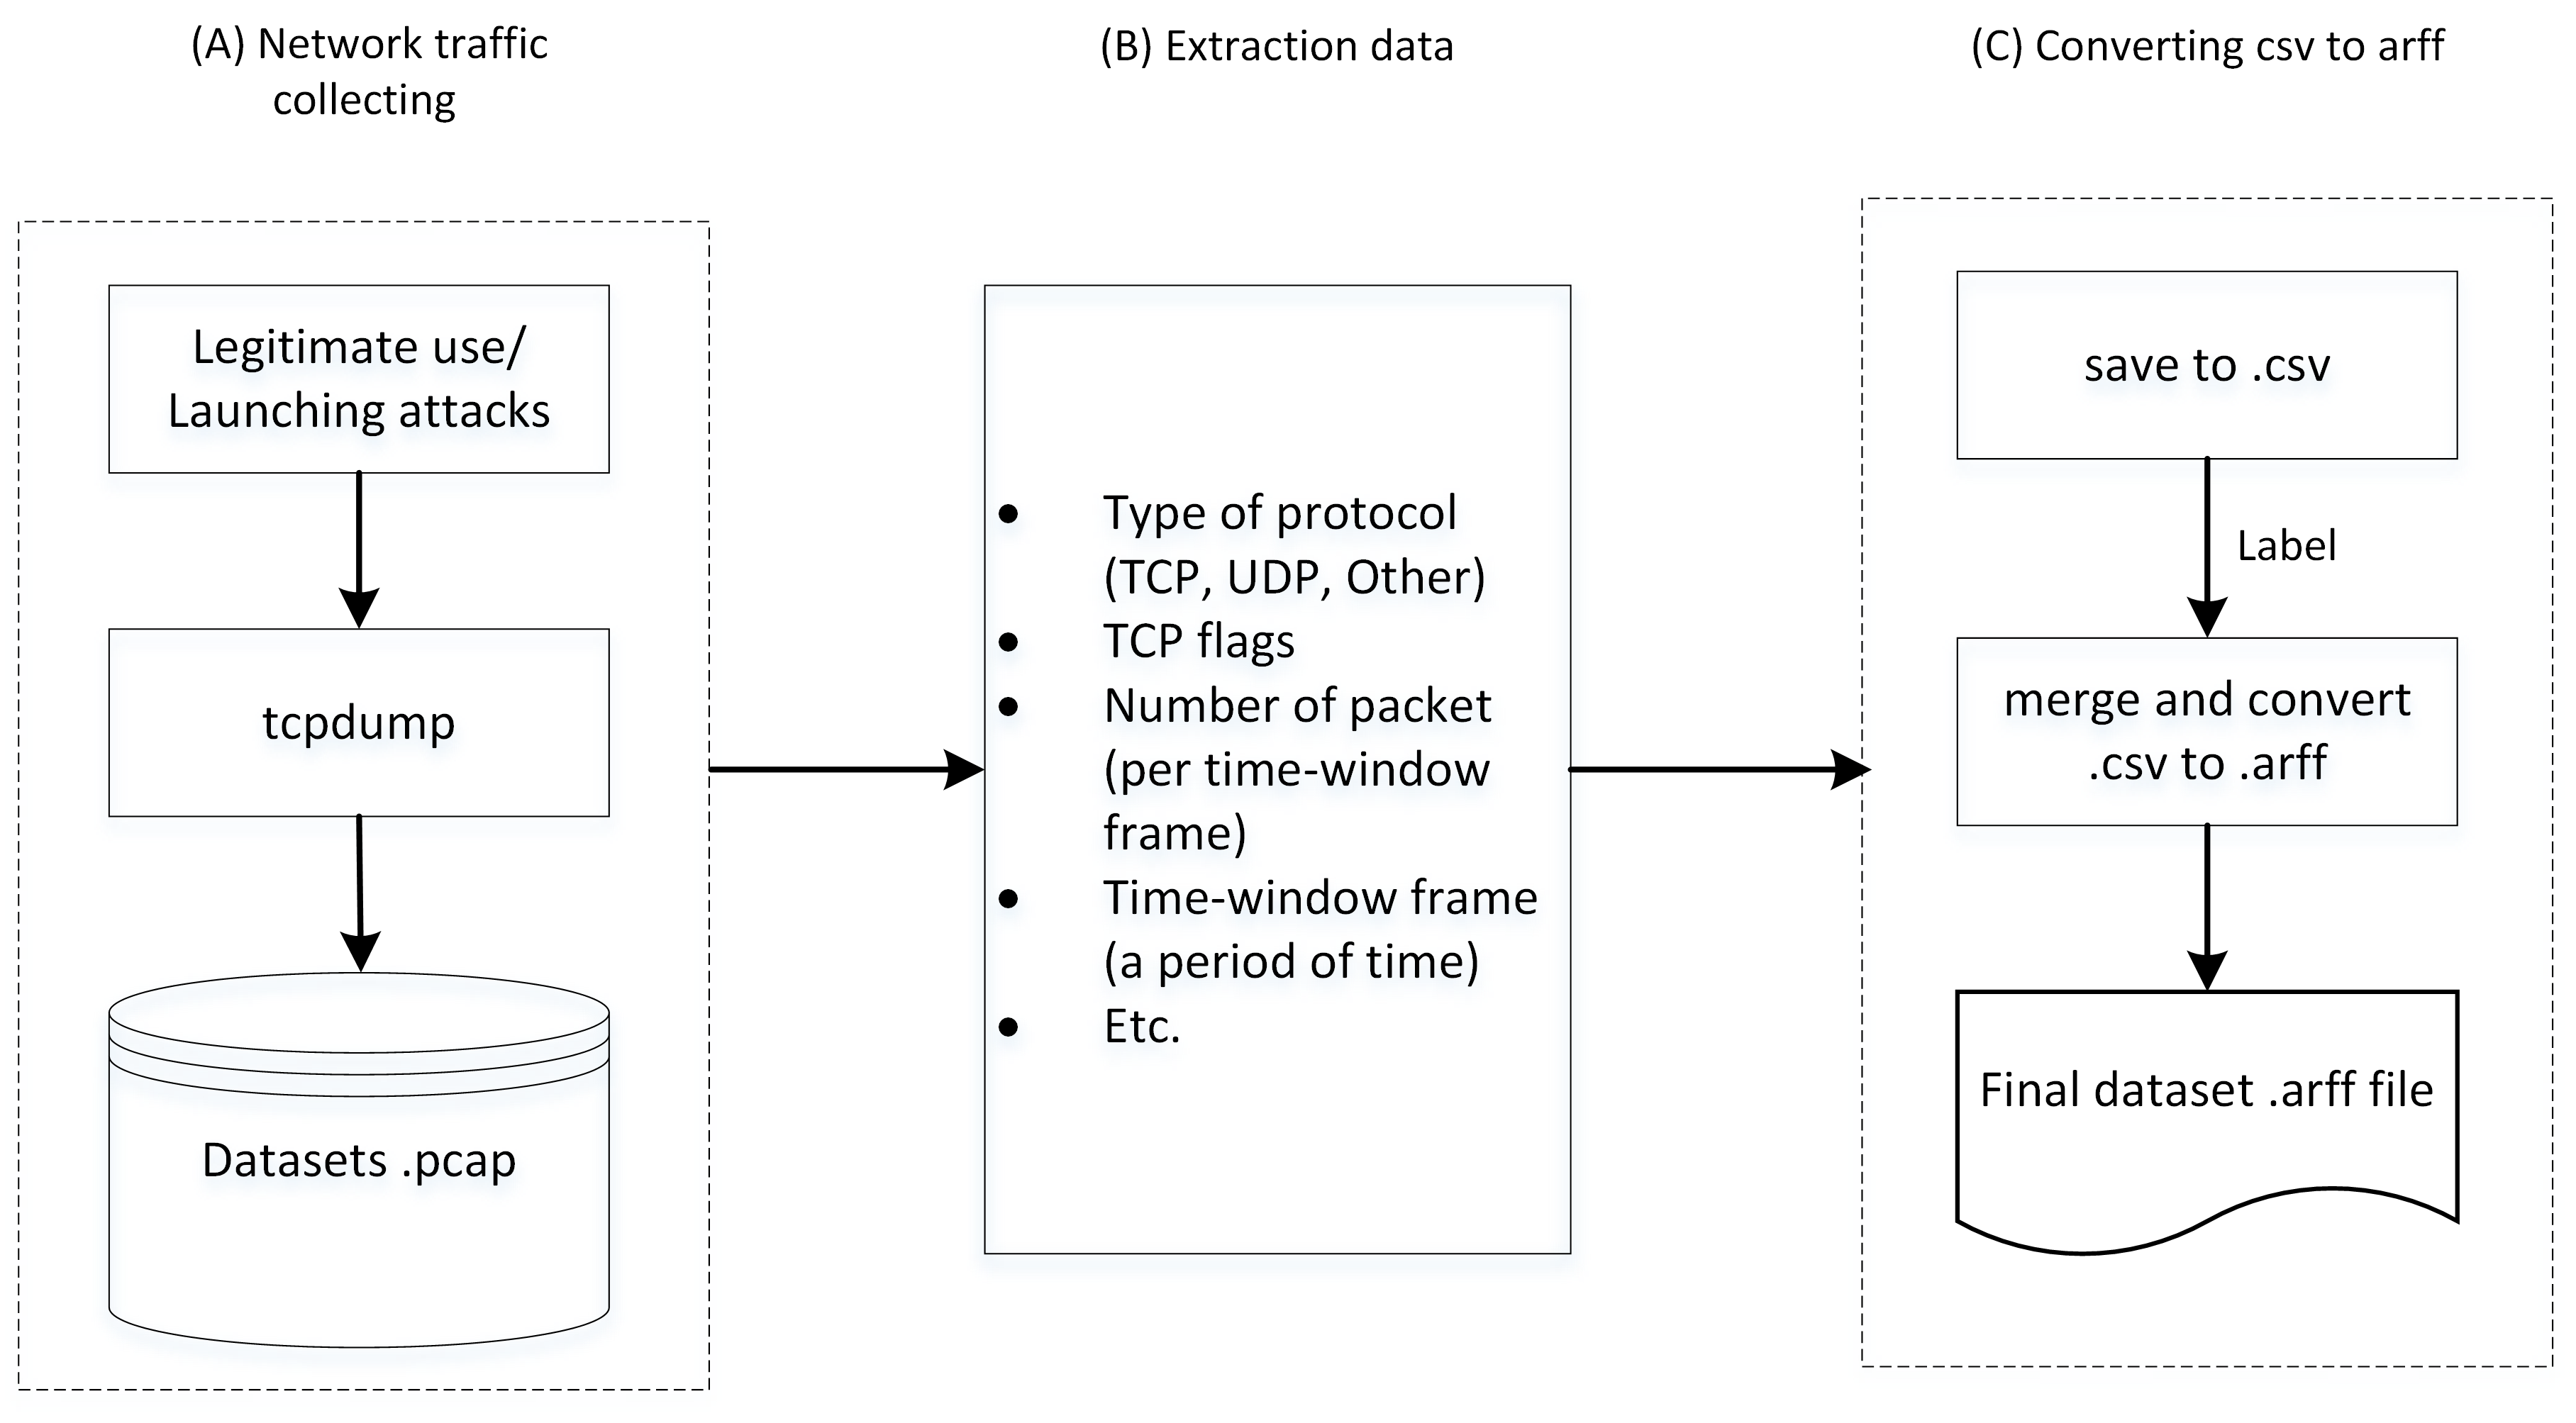
\includegraphics[width=\linewidth]{dataset_preparation_no_background.png}
\caption{Process of dataset preparation}
\label{fig:dataset_prepare}
\end{figure}

Each row in the final CSV represents a unique direction from source\_ip to destination\_ip for 4sec time window. The List of features which we covered in the dataset is shown in the Table
\ref{table:features} and the dataset preparation process is shown as Figure \ref{fig:dataset_prepare}.

\begin{table}
\begin{center}
\begin{tabular}{|p{3.1cm}|p{4.9cm}|}
\hline
\multicolumn{1}{|c|}{\bfseries Name of Feature} & \multicolumn{1}{c|}{\bfseries Description}\\
\hline
TYPE\_PACKET & Which type of packet – tcp, udp and other into string\\
\hline
FIRST\_TIMESTAMP & Arriving timestamp when the first packet received into numeric\\
\hline
NO\_OF\_PACKETS & No of packets how much received into numeric\\
\hline
DEST\_IP & Destination IP into string\\
\hline
SOURCE\_IP & Source IP into string\\
\hline
TCP\_FIN & Sum of TCP FIN flags into numeric\\
\hline
TCP\_SYN & Sum of TCP SYN flags into numeric\\
\hline
TCP\_RST & Sum of TCP RST flags into numeric\\
\hline
TCP\_PSH & Sum of TCP PSH flags into numeric\\
\hline
TCP\_ACK & Sum of TCP ACK flags into numeric\\
\hline
TCP\_URG & Sum of TCP URG flags into numeric\\
\hline
TCP\_ECE & Sum of TCP ECE flags into numeric\\
\hline
TCP\_CWR & Sum of TCP CWR flags into numeric\\
\hline
ETHER\_TYPE\_AVG & Average of Ethernet type into numeric\\
\hline
WIRELEN\_AVG & Average of Ethernet Wirelen into numeric\\
\hline
IP\_OFFSET\_AVG & Average of IP Offset value into numeric\\
\hline
IP\_LENGTH\_AVG & Average of IP Length value into numeric\\
\hline
IP\_VER\_AVG & Average of IP Version value into numeric\\
\hline
IP\_HLEN\_AVG & Average of IP hlen value into numeric\\
\hline
IP\_TTL\_AVG & Average of IP ttl value into numeric\\
\hline
IP\_FLAG\_AVG & Average of IP flag value into numeric\\
\hline
IP\_TYPE\_AVG & Average of IP type value into numeric\\
\hline
TCP\_OFFSET\_AVG & Average of TCP Offset value into numeric\\
\hline
TCP\_LENGTH\_AVG & Average of TCP Length value into numeric\\
\hline
TCP\_HLEN\_AVG & Average of TCP hlen value into numeric\\
\hline
TCP\_RESERVE\_AVG & Average of TCP Reserve value into numeric\\
\hline
TCP\_WINDOW\_AVG & Average of TCP Window size value into numeric\\
\hline
TCP\_URGENT\_AVG & Average of TCP Urgent value into numeric\\
\hline
PAYLOAD\_OFFSET\_AVG & Average of Payload Offset value into numeric\\
\hline
PAYLOAD\_LENGTH\_AVG & Average of Payload Length value into numeric\\
\hline
%ANOMALY\_SCORE & Class feature to label pattern (NORMAL/NMAP/DOS/R2L)\\
%\hline
\end{tabular}
\end{center}
\caption{Table of feature extraction}
\label{table:features}
\end{table}

We assume that all the packets which the direction from the Attacker to the target are abnormal then we labeled our dataset manually attacks and normal. After that, we merged and converted the dataset and 
converted into ARFF file format for development. We ignore and remove SOURCE\_IP, DESTINATION\_IP, and FIRST\_TIMESTAMP because we observe it somehow classified pattern by taking those specific values. So 
after removing those features we are just look at network behavioral features and extracting those to classify and generate Snort rule dynamically from the matched patterns.

\subsection{Data modeling and Machine learning}

Weka library is one of the famous open source library for data mining and machine learning \cite{misc:wekaTutorial}. It provides various algorithm and methods to work on any types of dataset to extract
useful features which can be applied to identify more accurately. Our research began with dataset preparation to build and train our model. We used ANOMALY\_SCORE class variable to predict a specific
pattern between normal and attack in the dataset. Decision tree is used where dataset has some predictor by which pattern can be classified into appropriate class. In our research we used J48 algorithm 
which is easy to convert into conditional algorithm for automatic Snort rule generation \cite{misc:weka.jar}. We used weka.jar library to implement J48 decision tree java program. Conditional program 
generated using weka by taking labeled training dataset as an input. It uses program template that we designed the Snort rule template with weka static method call which takes labeled/unlabeled testing 
dataset and generates Snort rules by looking at matched attack patterns and its classified feature values.

We used J48 decision tree machine learning algorithm to train the model as well as Snort rule generation by using that model \cite{NIDusingDT}. J48 decision tree classifier classify pattern by number of
feature from our dataset which we than converted into Snort rule using Snort rule template. For example if model classified a specific attack pattern by tcp\_syn, no\_packets and type\_packet features than
it will put those values of that specific features into the Snort rule template which we used in our NADIR application. Thus, we get the Snort rules as an output of the application.

%alert tcp \$EXTERNAL\_NET any -$>$ \$HOME\_NET any (msg: "[*] Attack-detected on S"; flags: S; flow: from\_client; threshold: type both, track by\_dst, count 182765, %seconds 4; sid: 3000001 ;)


\subsection{Snort configuration}

Intrusion Detection System (IDS) is a device which monitors packets on the computer networks. IDS reports attack behaviors based on rules and signatures applied to the machine. Intrusion Prevention System 
(IPS)  could achieve Real-time intercepting by leveraging in-line deployment in the network. It analyzes all network traffic passing through interface and takes actions to suspicious packets immediately
\cite{misc:netfilter}.

We converted Snort IDS into INLINE QUEUE mode using Iptables rules and Snort configurations. Now, it receives packets sent from the Net filter Queue with the help of the nfnetlink\_queue library 
\cite{misc:netfilter}. Snort compares the packets with Snort signature rules, takes action such as alert or drop if the packets are matched to a rule. Then, it finally sends them back to Net filter Queue 
where the Snort Inline tagged packets are processed. This effectively converts NADIR from passive IDS into an active IPS. 

%. An
%IPS (Intrusion Prevention System) where a packet matching a signature rule is blocked or modified.

In this case, the attacker will get the same information or fingerprints as the responses from the Vulnerable when the Attacker scans vulnerability services on the victim which are fake responses (replaced
payload packets). For example, the attacker gets a fingerprint of version of SSH service from the Vulnerable as SSH-2.0-OpenSSH-4.7p1 and gets the same information, SSH-2.0-OpenSSH-4.7p1, from Victim as
well even though the corrected information is SSH-2.0-OpenSSH-6.6.1p1 as shown in Figure \ref{fig:replacement}.

%\begin{figure}[h!]
%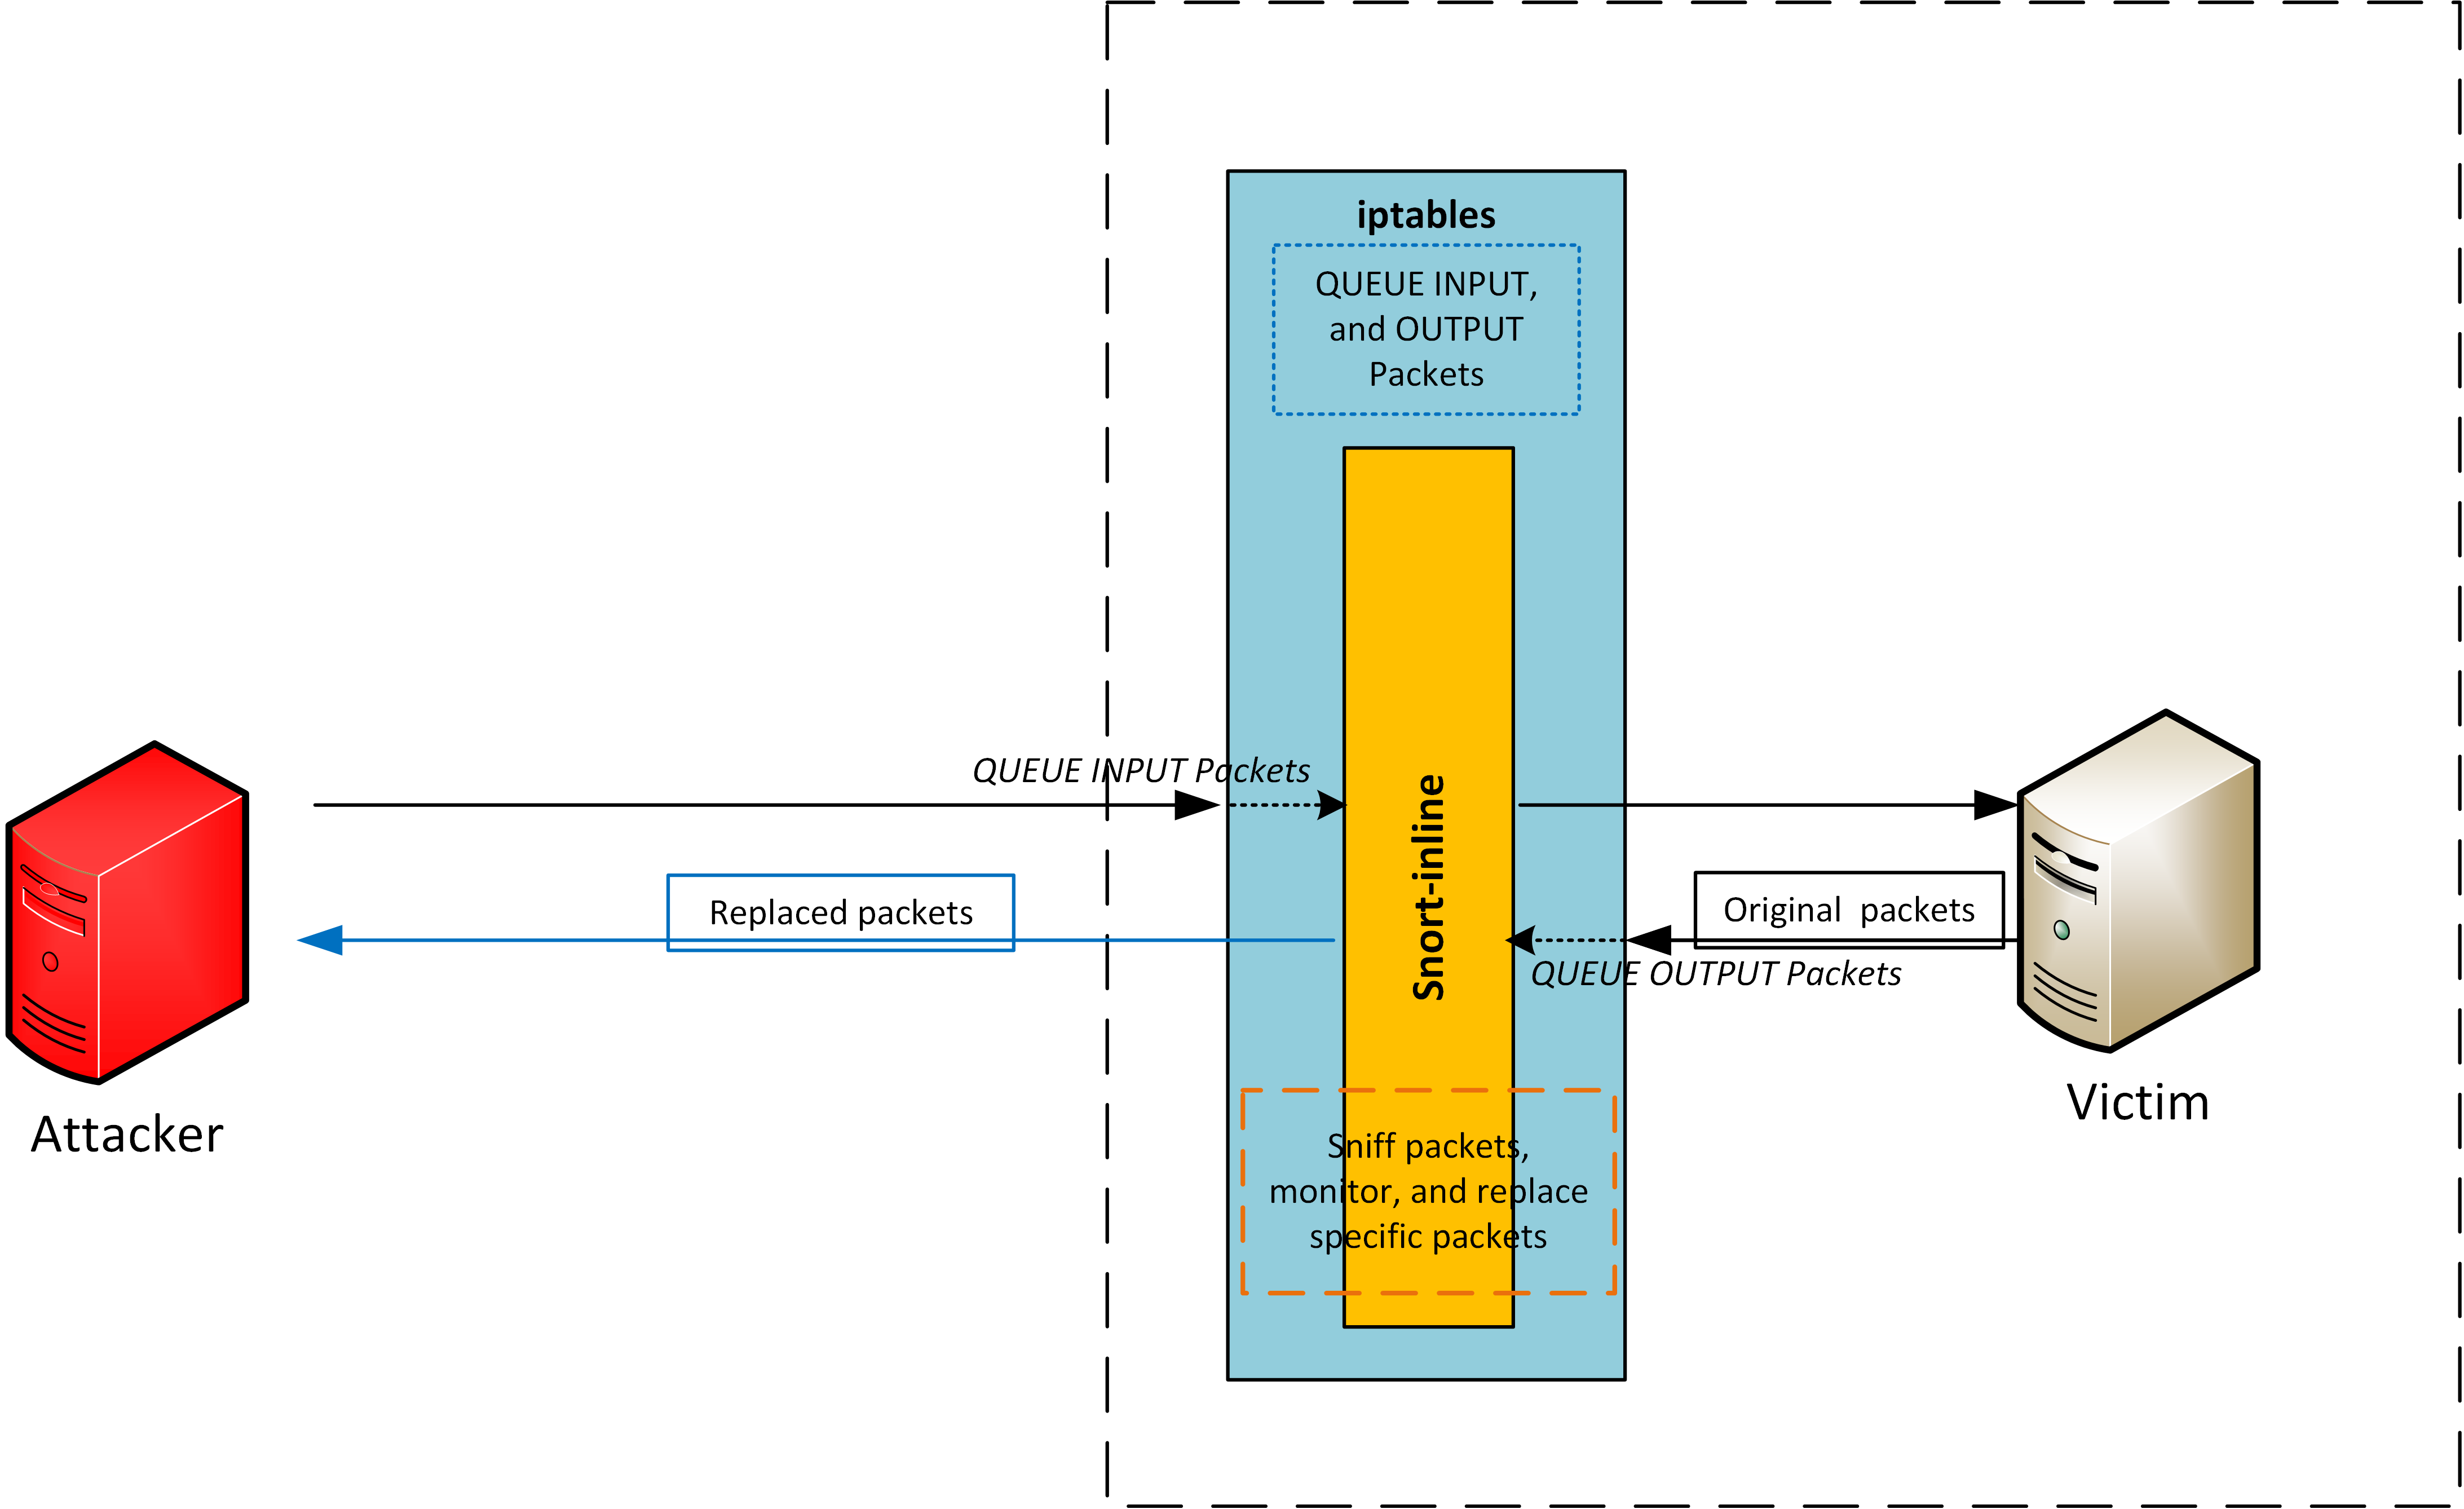
\includegraphics[width=\linewidth]{SnortProcessDiagram_no_back.png}
%\caption{Replacing payload model}
%\label{fig:replacementPayload}
%\end{figure}

%\noindent Figure \ref{fig:replacementPayload} shows how replacing process work on our model.

\begin{figure}
	\centering
	\begin{subfigure}[t]{1\linewidth}
            \centering
            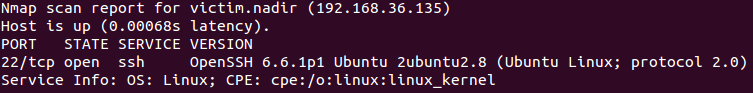
\includegraphics[width=\linewidth]{actual_print.png}
            \caption{The real running service information on the server}
            \label{fig:real_print}
	\end{subfigure}
	\vskip\baselineskip
  \begin{subfigure}[t]{1\linewidth}
            \centering
            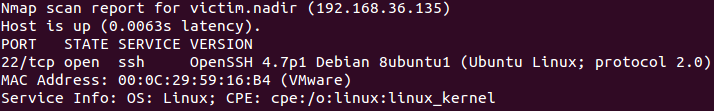
\includegraphics[width=\linewidth]{fake_print.png}
            \caption {The attacker gets the fake information}
            \label{fig:fake_print}
  \end{subfigure}
\caption{The figure show the service information that run on the server (a)Actual service version and (b)Fake service version}
\label{fig:replacement}
\end{figure}

In order to forge responses to service fingerprinting attempts, the first step is to queue all the packet not only from the attacker but also all the ingress/egress traffic by iptables. Then, all the
traffic will pass through the Snort which run as inline mode. The input traffic packets will not be replaced the payload yet, Snort just only monitors the traffic and tries to match with the Snort rule. 
Once the input packets are match with the rule, Snort will replace the content of the payload of the original response packet to be pre-payload which is same as vulnerable response. Lastly, the replaced 
packets that contain a fake response will be sent back to the attacker. Thus, the attacker will learn and get an incorrect information.

\subsection{Overall system setup}

The over-all process of NADIR system is show as Figure \ref{fig:overall}. As development phase of this research, we rebuild the whole system by reconfiguring Snort and adding Snort rules to replace
payloads by checking the TCP flags of incoming requests \cite{misc:snortflowbit}. We divide Snort rules into four different rule files: (1) my-flowbits.rules, (2) my-print.rules, (3) my-snort.rules, and (4) my-drop.rules

The (1) my-flowbits.rules and (2) my-print.rules which we developed at beginning are used to control the process of replacement of any string or payload. The other rule files will be maintained by the NADIR application. At the end, we come up with the overall system setup with our NADIR application which takes training labeled dataset and unlabeled or labeled testing dataset to generate the decision tree by using J48 algorithm then generating Snort rules dynamically based on the decision tree. The NADIR application generates Snort rules and updates my-snort.rules file by inputting the training/testing dataset. The NADIR application tracks the Snort logs and it generates filtering rules and update my-drop.rules file if an attack happened and detected. After successfully updating the Snort rules, we managed daemon to restart the Snort service without
missing any packets by using two different daemon services and two Snort instances To handle two Snort instances we used two bridge interfaces. If the first Snort instance is running and the Snort
rules need to be updated, the NADIR application runs another Snort instance with updated rule sets and halts the first Snort instance. NADIR also flushes the entire drop rule file every night and keep the all blacklist IPs into backup file automatically so that we can have the benefit of temporary blocking.
